\documentclass{VUMIFPSbakalaurinis}
\usepackage{float}
\usepackage{hyperref}
\usepackage{algorithmicx}
\usepackage{algorithm}
\usepackage{algpseudocode}
\usepackage{amsfonts}
\usepackage{amsmath}
\usepackage{bm}
\usepackage{caption}
\usepackage{color}
\usepackage{graphicx}
\usepackage{listings}
\usepackage{subcaption}
\usepackage{wrapfig}
\usepackage{biblatex}
\usepackage{microtype}

% Titulinio aprašas
\university{Vilniaus universitetas}
\faculty{Matematikos ir informatikos fakultetas}
\institute{Informatikos institutas}  
\department{Programų sistemų studijų programa}
\papertype{Bakalauro baigiamojo darbo planas}
\title{Vaizdo žaidimo eismo vaizdų generavimas naudojant nesuporuotų vaizdų transformacijas}
\titleineng{Video game traffic image generation using unpaired image to image translation}
\status{4 kurso 5 grupės studentas}
\author{Gytis Oksas}
\supervisor{j. asist. Boleslovas Dapkūnas}
\reviewer{doc. dr. Linas Petkevičius}
\addsignatureplaces{} % prideda parašų vietas tituliniame puslapyje
\date{Vilnius – \the\year}

\bibliography{bibliografija}

\begin{document}
\maketitle

\sectionnonumnocontent{Įvadas}
    Vaizdų transformacija (angl. \emph{image-to-image  translation}) yra plačiai taikoma metodika kompiuterių regos ir paveikslų apdorojimo problemoms spręsti \cite{ImTImTr}. Metodai, sprendžiantys šias problemas, gali būti taikomi parinktų specifinių paveikslėlių požymių keitimui, trūkstamų paveikslėlio pikselių užpildymui arba realistinių vaizdų generavimui. Ši taikymo sritis gali būti naudinga kuriant žaidimų meninį turinį (pavyzdžiui, tekstūras, realistinių objektų dizaino atitikmenis žaidimui), kuriant animacijas. Ir nors realių vaizdų transformavimas į nerealistinių vaizdų domeną nėra naujas (pavyzdžiui, veido nuotraukas transformuoti į animacinių filmukų stilių, kaip yra taikoma MSPC modelio pavyzdžiuose \cite{Mspc}), jis vis dar yra aktyviai analizuojamas, kadangi yra likusių ir pastoviai iškylančių problemų ir iššūkių (pavyzdžiui, vaizde daug triukšmo, besikartojantys artefaktai, nelogiški piešiniai). Vaizdo žaidimų vaizdų transformavimas į realistinius vaizdus yra spręstas, tačiau atvirkštinis variantas yra gan mažai išnagrinėtas.

    \begin{figure}[H]
        \centering
        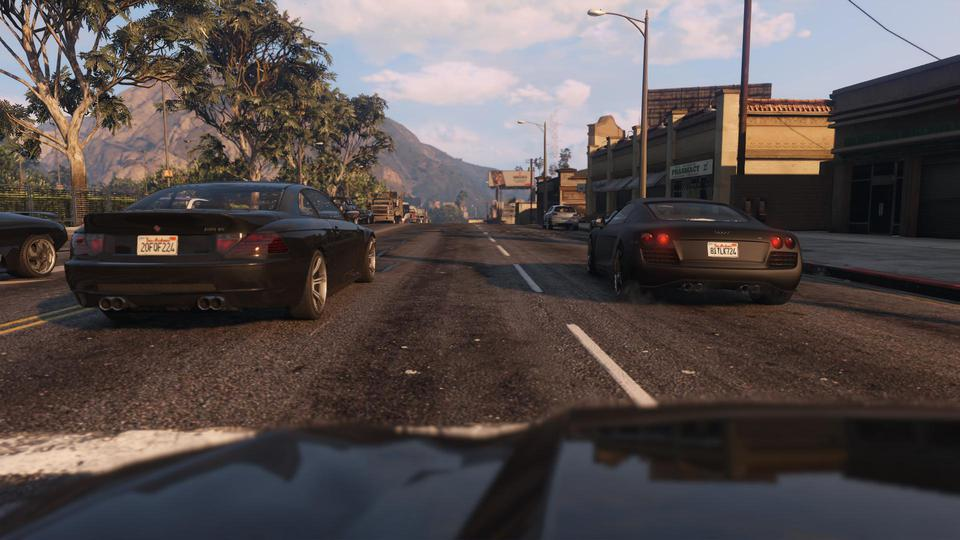
\includegraphics[scale=0.3]{img/EnPhEn_before}
        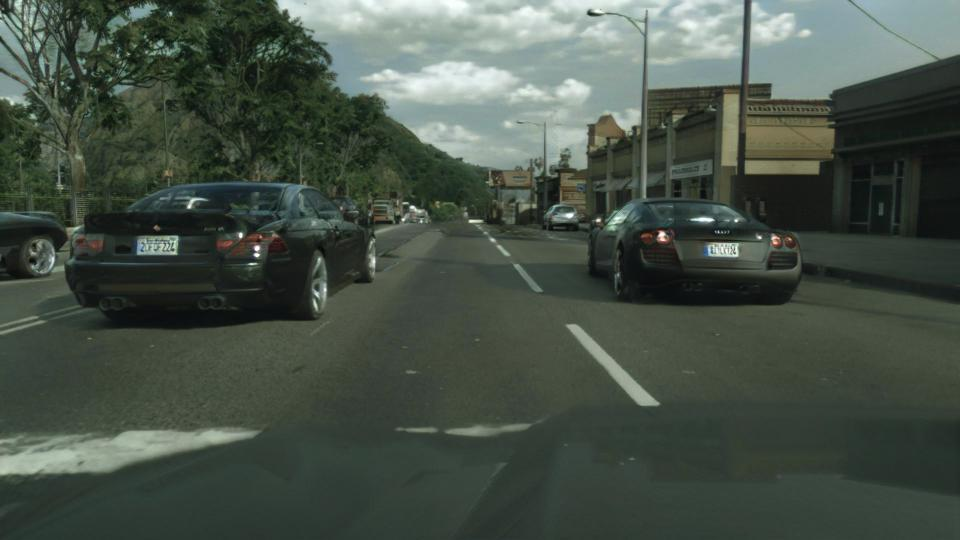
\includegraphics[scale=0.3]{img/EnPhEn_after}
        \caption{Vaizdai prieš ir po nuotraukos transformavimo, atitinkamai.\cite{EnPhEn}}
        \label{img:mlp}
    \end{figure}
    
    Tyrimas kuris atkreipė daug dirbtinio intelekto ir vaizdo žaidimų mėgėjų dėmesį yra aprašytas Intel dirbtinio intelekto mokslininkų straipsnyje „Enhancing Photorealism Enhancement“ \cite{EnPhEn}, jame pristatomas metodas, kaip išnaudojus modernias dirbtinio intelekto technologijas yra sukuriamas nuotraukų transformatoriaus modelis, sugebantis žaidimo GTA V automobilių eismo vaizdus paversti foto realistiniais, lyg įrašytais automobilio registratoriumi. Jis vienas pirmųjų įtikinamai, švariai, be prarastų esminių nuotraukų detalių ir be pridėtinių artefaktų sugebėjo transformuoti nuotrauką į realistiškai atrodantį vaizdą (žr. 1 pav.). Tai davė idėją šiam tyrimui – apsukti puses ir sukurti modelį, kuris pagal tuos pačius atributus sugebėtų transformuoti realybės automobilių eismo vaizdus į vaizdo žaidimo automobilių eismo vaizdus.

    \subsubsection*{Tyrimo metodai ir laukiami rezultatai}
        Kursiniame darbe buvo panaudoti, jau tapę tradiciniais, generatyviniai adversariniai tinklai \cite{OrigGan} (angl. \emph{generative adversarial network}), kurie turėjo savo trūkumų su turinio dingimu po nuotraukos transformacijos (daugiausiai iš nuotraukų buvo ištrinti automobiliai), todėl svarbi tyrimo dalis bus sukurti metodą, leidžiantį atskirti bendrą turinį ir dingstančias klases iš vaizdo (naudojant segmentacinius modelius) ir taip atskirai transformuoti bendrą vaizdą ir dingstantį turinį (t.y. automobilius), ir šiuos vaizdus algoritmiškai sujungti. Šio metodo norimas rezultatas yra kokybiškas foninių detalių transformavimas su išsaugomais automobiliais nuotraukose, t.y. kelių modelių programa, kuri sugeba išsaugoti daugiau detalių nei pavienis MSPC modelis \cite{Mspc} (apmokytas kursinio darbo metu) be papildomos logikos ar skaičiavimų.
    
        Pastaraisiais metais taip pat pradėjo populiarėti difuziniai nuotraukų generavimo modeliai \cite{DiffMod}. Jie sugeba kurti nuotraukas su kur kas mažiau triukšmo ir įtikinamesniu turiniu, tačiau šių modelių mokymas ir naudojimas trunka kur kas ilgiau. Dėl šių priežasčių, dalis darbo gali būti skiriama bandymams, ar šie nauji modeliai gali būti pritaikyti ir gali būti naudingesni nei įprasti GAN modeliai, šios užduoties scenarijuje. Norimas rezultatas iš šio eksperimento būtų kokybiškiau arba švariau (mažiau artefaktų, nuotraukos triukšmo) transformuotas vaizdas.

    \subsubsection*{Darbo atlikimo procesas}
        \begin{enumerate}
            \item Sukurti vaizdo žaidimo automobilių duomenų rinkinį.
            \item Apmokyti MSPC modelį transformuoti tik automobilių nuotraukas
            \item Kursiniame darbe apmokytą bendrą MSPC modelį ir MSPC automobilių nuotraukų transformavimo modelį apjungti programoje, kuri naudojanti segmentacinį modelį atskirtų automobilius iš nuotraukos, transformuotų abi nuotraukas ir įklijuotų transformuotą automobilio nuotrauką atgal į bendrą nuotrauką. 
            \item Rasti ar yra difuzijos modelių sugebančių transformuoti nuotraukas tarp dviejų domenų naudojant nesuporuotų nuotraukų transformaciją, jei rasti pavyktų, apmokyti difuzinį modelį su turimu duomenų rinkiniu.  
            \item Palyginti ar naujų modelių rezultatai yra geresni negu kursiniame darbe gauto modelio (atsižvelgiant į naujesnių metodų kompleksiškumą ir didesnes sąnaudas).
        \end{enumerate}

    \subsubsection*{Darbo tikslas}
        Šio tyrimo tikslas ir yra sukurti metodą, gebantį transformuoti realias eismo nuotraukas į vaizdo žaidimo vaizdus, tačiau neprarandant esminių semantinių objektų (šiuo atveju - automobilių). Pasirinkta buvo transformuoti nuotraukas į  žaidimo „Grand Theft Auto: Vice City“ (toliau trumpinama „GTA:VC“) domeną dėl jo išskirtinio meninio stiliaus ir ryškaus domeno požymių skirtumo lyginant su realaus eismo nuotraukomis. Tyrimo uždaviniai:
        \begin{enumerate}
            \item Sukurti vaizdo žaidimo duomenų rinkinį.
            \item Sukurti vaizdo žaidimo automobilių duomenų rinkinį.
            \item Sukurti metodą sugebantį atskirai transformuoti tam tikrą nuotraukos semantinę klasę ir gautą rezultatą atgal įklijuoti į nuotrauką. 
            \item Palyginti modelius.
        \end{enumerate}

        \nocite{*}

\printbibliography[heading=bibintoc]

\end{document}
